\section{Liquid State Machine (LSM)}
Sıvı Hal Makinesi (Liquid State Machine), sinir ağlarının öğrenme ve işleme yeteneklerini sıvı içeren bir sistemle birleştirerek işlem yapar. Temel bileşenleri:
\begin{itemize} 
    \item \textbf{Sıvı (Liquid):} Sıvı haldeki bir medya veya dinamik birliklerin oluşturduğu bir ortamdır.
    \item \textbf{Dinamik Birlikler (Dynamic Units):} LSM içindeki sinir hücrelerine denir. 
    \item \textbf{Giriş ve Çıkış Katmanları:} Dış dünyadan gelen girişleri alıp sonuçları çıktı olarak veren katmanlardır.
\end{itemize}

\begin{figure}[h]
    \centering
    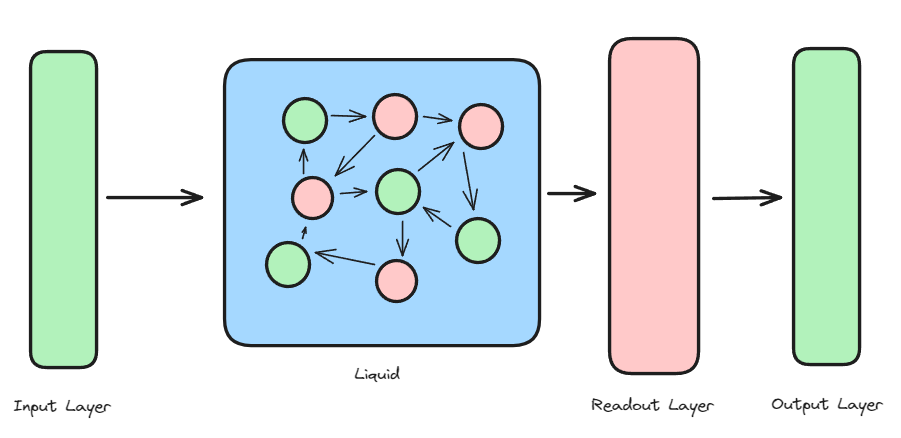
\includegraphics[width=1\textwidth]{images/liquid_state_machines.png}
    \caption{Sıvı hal makinesi mimarisi.}
    \label{fig:enter-label}
\end{figure}

\subsection{Çalışma Adımları}
\begin{enumerate}
    \item Giriş verisi, giriş katmanından alınarak sıvıya iletilir.
    \item Giriş verisi, sıvı içerisindeki dinamik birimler tarafından işlenir. Sıvı, birbiriyle etkileşim için karmaşık halde dinamik birimlerden oluşur. Girdi, sıvı içinde yayılır ve işlenir.
    \item Giriş verisi zamanla sıvı içinde dolaşır ve işlenir. Bu işlem, zamansal bilgi işleme yeteneği sağlar.
    \item İşlenen veri çıkış katmanına sunulur.
\end{enumerate}

\newpage